
\section{Selecting Platforms in CLIC}
The platform selection is to find the platform with the lowest cost for each logical operator in the logical plan. We take this problem as a node classification problem, where the platform of the lowest cost is considered as the label of the logical operator. We use the GCN as the classifier, which is considered more suitable for node classification problems. Below we first narrate the feature extraction method used in CLIC and then describe the classification method using GCN.

\subsection{From One-hot Encoding To Embedding}
The traditional one-hot encoding method used in [rheem, ml-based] to treats each operator as a dimension to vectorize the operator as a 0-1 vector. 
Its dimension equals to the number of operators and each vector only has one non-zero value, therefore the one-hot encoding is always high-dimensional and sparse. 
Generally speaking, this methoid is less computational since the majority of neural network toolkits do not play well with very high-dimensional, sparse vectors [Neural Network Methods in Natural Language Processing, 2017].

Besides, the one-hot encoding is imcompatible to a new operator which goes against our high extensible character. 
In particular, the one-hot encoding needs to increase the dimension of all operator vectors whenver a new one is inserted. 
Figure xx examplified this situation where as the new Flatmap operator (red one) being inserted, all the vectors' dimension are grown. 
Thus the previous model needs to be retrained otherwise the new vector becomes an invalid input due to its higher dimension. 
Even if reserving some empty dimension to stablize the input, the model still cannot properly classify the new operator because the new dimension is orthogonal to the other dimension and the model lacks knowledge about this new dimensions.

In order to overcome the above two problems, we turned our attention to using the embedding to represent the operator. 
In mathmatic, an embedding is a function f X -> Y that maps a data point X in one space to point Y in another space. 
This is the most important preprocess technique in natural language processing (NLP), where the word embedding is a term used for the representation of words for text analysis. 
It is typically in the form of a real-valued vector that encodes the meaning of the word such that the words that are closer in the vector space are expected to be similar in meaning [wiki]. 
For promotion, there also are image embedding, video embedding, and of course, operator embedding. 

The Operator embedding is a representation of an operators in the Euclian space. 
We can share the same idea in the word embedding that allows semantically similar operators to have closer distance. 
Figure xx outlines the embedding structure. 
It can be seen that (i) the dimension of the vector space is independent of the number of data points and is usually much smaller than that of the one-hot encoding []. 
In short, the embedding is dense and low-dimensional, therfore more computational; 
(ii) the embedding of the old and new operators are in the same Euclidean space and the embedding includes the semantic relationship of the operators, 
therefore the model can make inference directly for the new operators using the existing knowledge. 

\begin{figure}
    \subfigure[One-Hot Encoding]{
        \label{fig:one-hot}
        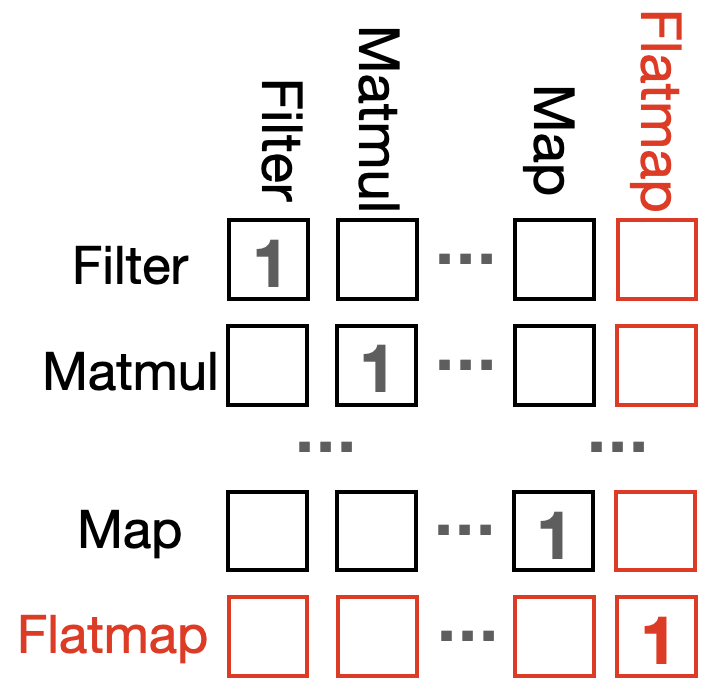
\includegraphics[width=0.3\linewidth]{figures/one-hot.png}
    } 
    \subfigure[Operator Embedding]{
        \label{fig:embedding}
        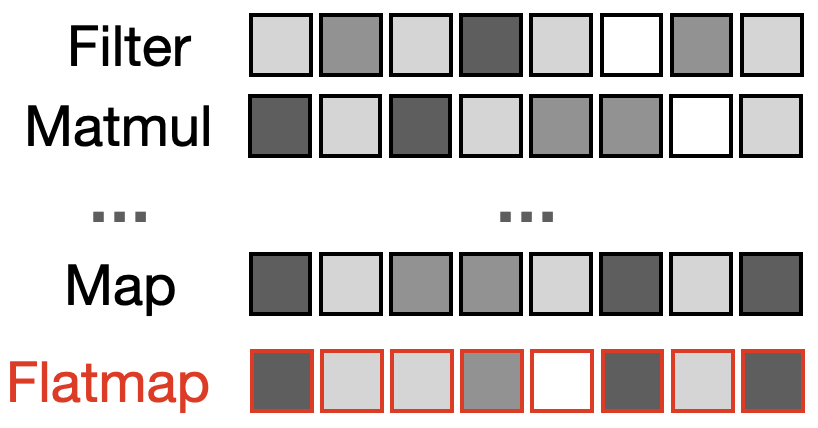
\includegraphics[width=0.3\linewidth]{figures/embedding.png}
    } 
    \caption{Vectoization Method}
    \label{fig:encoding}
\end{figure}


\subsection{GCN Intuition}
Graph Convolutional Network is a convolutional neural network that can be directly applied to graphs. 
It stacks layers of learned first- order spectral filters, which are followed by an activation function to learn graph representations [42].

‘Convolution’ in GCN refers to multiplying the input matrix with a set of weights that are commonly known as filters or kernels. 
The filters act as a sliding window across the matrix and enable GCN to learn features from neighboring cells. 
Before convolution, there needs a extra normalization step to change the irregular topology into matrix. 
Figure XX shows the node classification process of one operator using GCN. 
It first traverses each operator in the logical plan and samples K (a hyperparameter) neighboring operators to form a K*|V| matrix where E indicating the length of operator's feature vector. 
If the operator has less than K first-level neighbors, then it adds second-level neighbors. 
Then it applys the kernel across the matrix and gets the vector that contains the topological information. 
After that, the vector is fed into the neural network to compute its graph representation that can be used to classify. 
Finally, we use the MLE as the loss function to compare the graph representation and the platform embeddings and update the GCN.


\begin{figure}
  \centering
  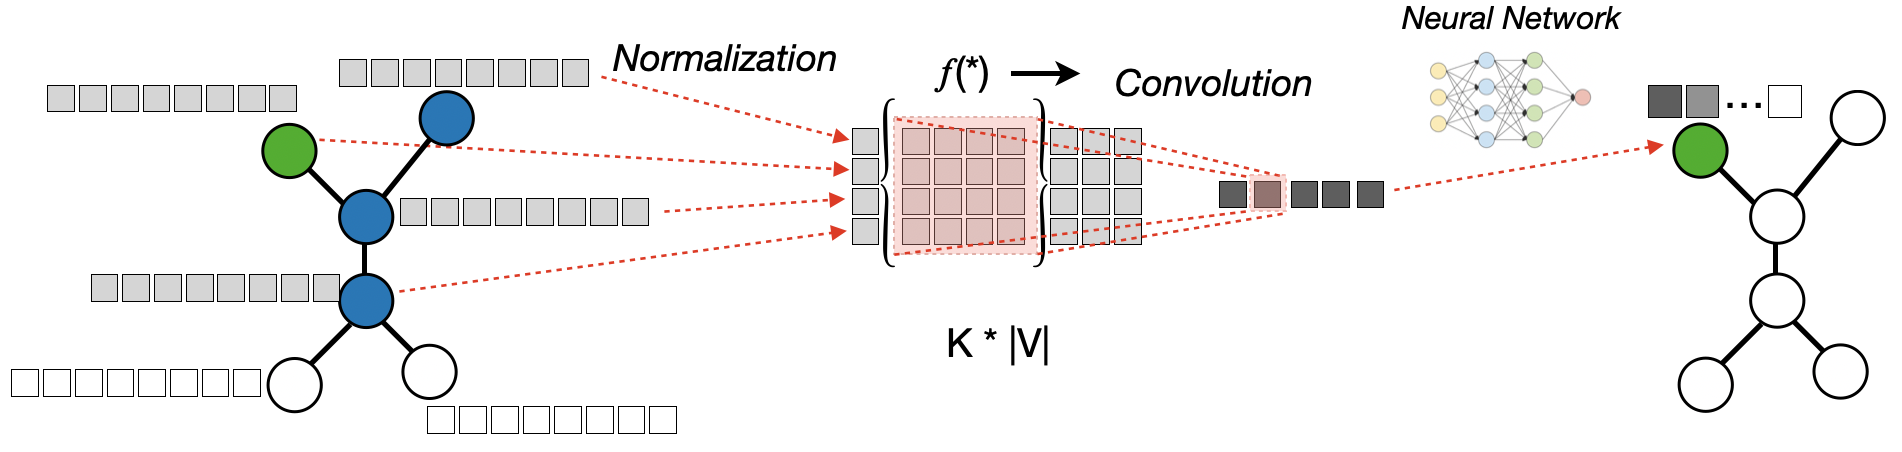
\includegraphics[width=\linewidth]{figures/gcn.png}
  \caption{Selecting platforms with GCN}
  \label{fig:gcn}
\end{figure}

\subsection{Data Generation}
\textbf{Generating Operator Embedding}
In word embedding, because the words in a sentence have certain correlation with its context words, 
therefore the cost function of training Word Embedding is to maximum the joint probability of the word and its context words. 
Similarly, we can also reasonably assume that the operators that appear in a same logical plan have more association and use the same cost function. 
We take the topological-ordered logical plan as the sentence and the logical operators inside are words, 
then use the same model to train the operator embedding. The results are shown in Figure xx. 
For the sake of visualization, we just show the top-2 dimensions with the highest eigenvalue. 
One observation is that operators that are the same computing paradigm and have the same number of inputs and outputs tend to have small cosine distance. 
What's more, the newly inserted Flatmap operator is also mapped closer to the Map operator instead of the Matmul operator which is probably due to the same reason.

It's important to emphasize that the operator embedding technique is not bound with CLIC but a general feature extraction method. 
One can generate an operator embedding whether the operator is supported by CLIC or not as long as there are logical plans that contain this operator.

As we have mentioned that the operator embedding is compatible for the newly integrated operator. 
There're two cases when integrating a new operator:
\begin{itemize}
    \item [1)]
    The operator is new to CLIC but not the model, therefore its embedding can be retreived in CLIC directly from the model.
    \item [2)]
    The operator is also new to the model, i.e. the "OOV" (out of vocabulary) problem. 
    In this case, the model needs some new training data to recognize it. 
    Therefore, we synthesize some new logical plan that contains the operator according to operator's attributes and then incrementally updates the model to generate the embedding.
\end{itemize}

Apart from the above operator embedding, 
we also design and generate the embedding for each physical computing platform. 
The mathmatical meaning and generation method goes the same. 
We don't further explain due to limits of space.


\textbf{Generating Training Data}
The effectiveness of the GCN strongly depends on the training data. 
In our case, a large amount of disparate logical plans (data points) together with the best physical platform (labels) of each logical operator in it is required. 
The logical operator's feature vector is composed of two parts: operator embedding and the global hardware resources. 
The latter is the same for the operators in the same logical plan, including infrastructure's CPU frequency, main memory, GPU memory, network bandwidth, etc. 
However, there is currently a lack of the Workflow dataset for cross-platform computation, so we borrow the TDGen [] to synthesized datasets separately for each computation mode and on different infrastructures.